\chapter{Conclusions and Outlook}

\label{Chapter5} % Change X to a consecutive number; for referencing this chapter elsewhere, use \ref{Chapter5}

Throughout this work, I have sought to understand the intrinsic
structure of machine-learning models and how this gives
rise to adversarial attacks. I began by studying the construction of
neural networks in Chapter~\ref{Chapter1} and learning in practice by generating adversarial
attacks in Chapter~\ref{Chapter2}. This led naturally to a more careful study of decision
boundaries and the development of the Persistence metric in Chapter~\ref{Chapter3}. Uncanny drops in persistence while crossing
decision boundaries toward adversarial attacks indicated that attacks
may exist in highly curved regions. The field conspicuously lacks
tools for evaluating curvature, although some progress is being
made. In the process of searching related work for methods that would allow more
direct analysis I discovered deficiencies in nascent literature on
path kernels starting with the work of ~\citet{domingos2020}. The
initial work to correct these deficiencies and produce an exact path
kernel are presented in Chapter ~\ref{Chapter4}. This new exact path kernel
representation for neural networks has a primary advantage which is to
decompose model predictions into contributions from each training
point. We can use this representation to decompose predictions into
parameter gradient contributions from each training datum, thus the exact path kernel implicitly maps the
training data into a given tangent space. This mapping can be done for
parameter gradients, input space gradients, and several other
spaces related to both of these. Two such decompositions are applied
in Chapter~\ref{Chapter4a} to demonstrate that many cutting edge OOD
detection algorithms implicitly use this decomposition in terms of
parameter gradients, and that training input gradients can be
used to measure signal manifold dimension.

We can summarize the first 3 Chapters as posing some fundamental
geometric questions related to machine-learning robustness. 
Chapters 4 and 5 as propose a new framework for analyzing geometric
properties and demonstrating that this framework can be applied very
generally. As usual in mathematics, trying to solve a specific problem
about geometric causes for adversarial examples has led to a very
general result in a totally different field. Although Chapters 4 and 5
represent significant progress in understanding ANNs mathematically,
they do not directly address the core question that arose within the
first three Chapters: Is relative dimension and curvature a primary
cause of adversarial vulnerability. 

Based on this work, we can now make some supportable conjectures:

\begin{enumerate}
  \item Modern neural network architectures learn decision boundaries
    that are askew from many interpolations among training and testing
    data.
  \item Non-orthogonal decision boundary crossings indicate that
    sharp corners in the decision space learned by ANN models lead
    to adversarial examples.
  \item Bilinear map based representations allow decomposition of
    predictions based on training inputs. These show that models
    implicitly use a lower dimensional implicit representation of data
    to make predictions.
\end{enumerate}

Combining these notions, we have a clear path forward:
    Decompose adversarial attacks using a bilinear map
    representation and then compare these signatures of variation with
    typical modes of variation within training data.
Likely this will show that adversarial attacks are arising
    from sharp corners in decision space, some of which can be
    mitigated by making models more aware of the properties of the
    decision space they have learned, some of which cannot be
    mitigated because training data are insufficient to fully
    constrain decision surfaces. 
From here, there are several important directions for
future research. First is the application of these methods directly to
the adversarial robustness questions from Chapters 1-3. Second is the
complete generalization of this new framework including conditions
under which such representations live in Banach spaces or Hilbert
spaces and what order of accuracy can be maintained using truncated
singular value decomposition. Third is the application of this theory more
broadly to connect with Wasserstein metric spaceswhich is a suspected implicit space learned by machine-learning models. 

\section{Applications to Adversarial Robustness}

\begin{figure}[ht!]
    \centering
    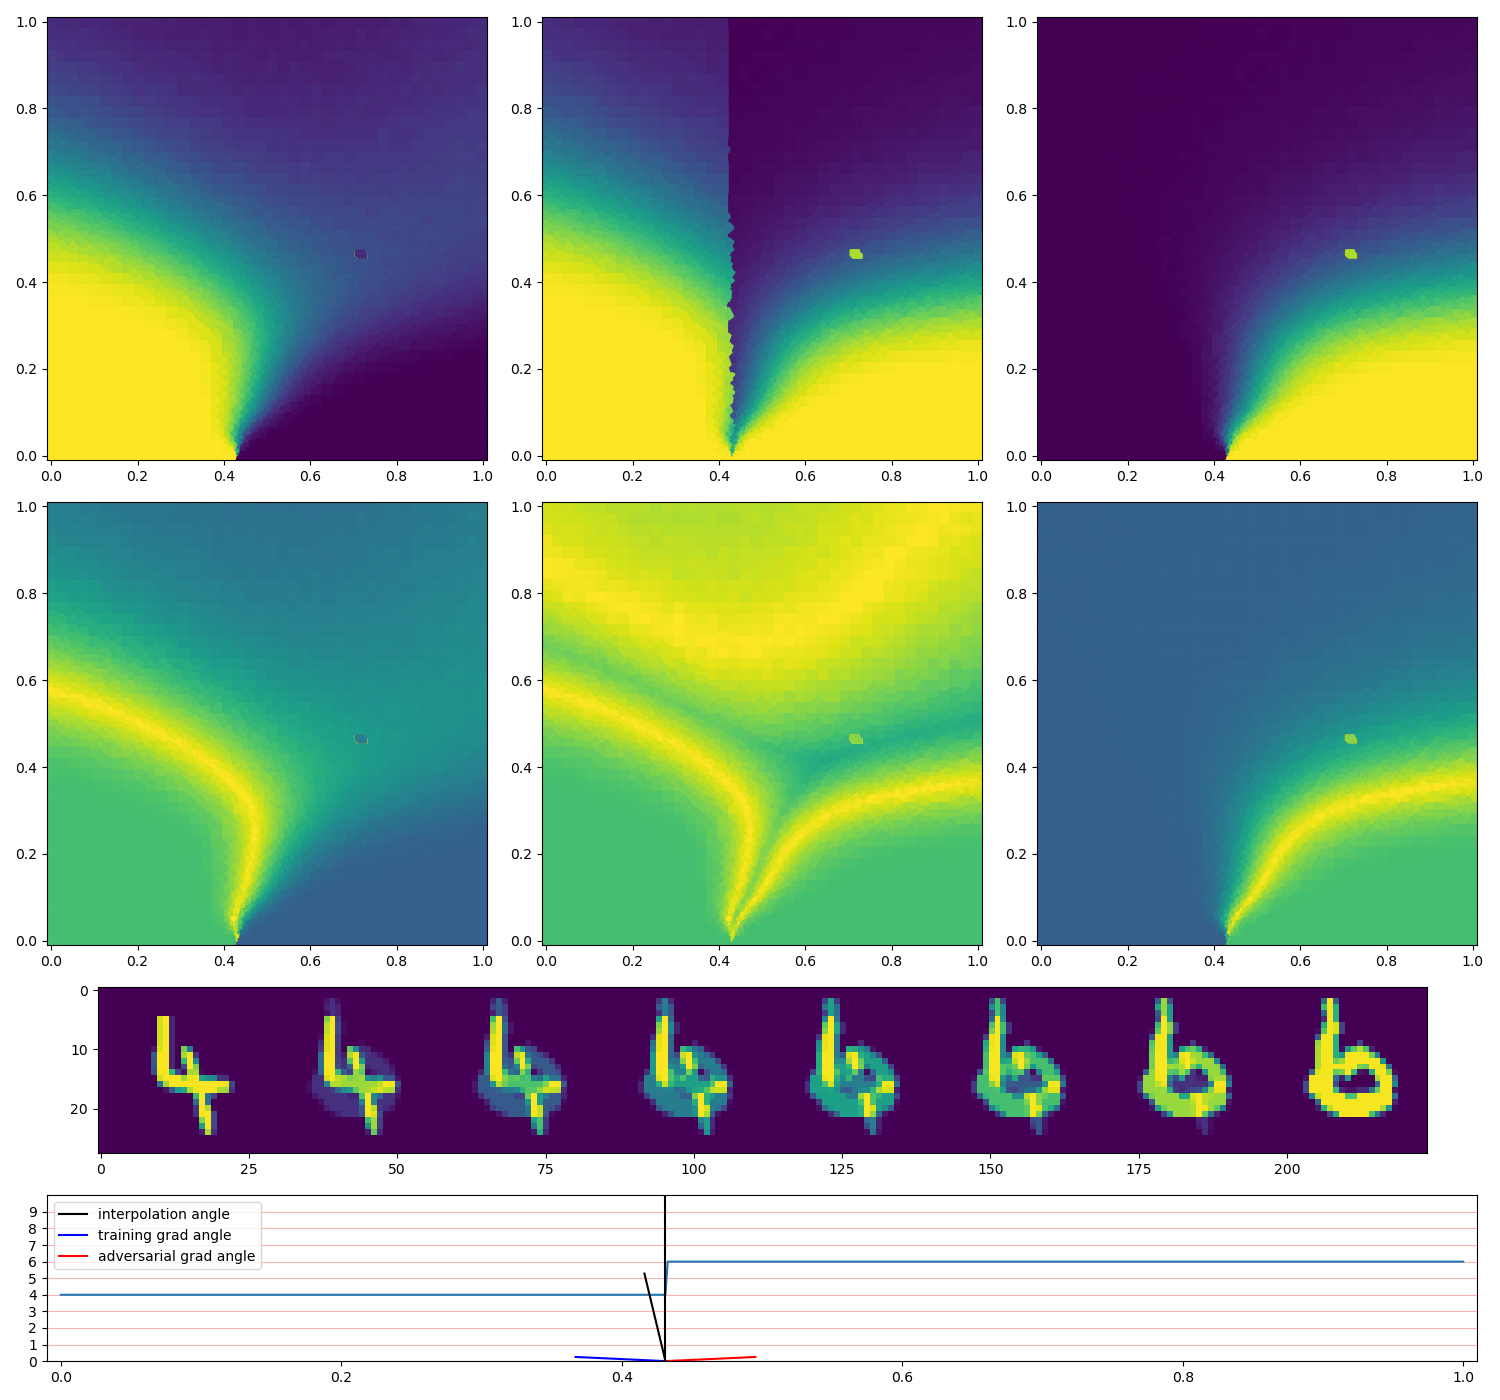
\includegraphics[width=0.42\textwidth]{c5_figures/stab-mnist-C32-50-50-10-0.001-eval-1e-06-none-4-6-db_interp-stability-50.png}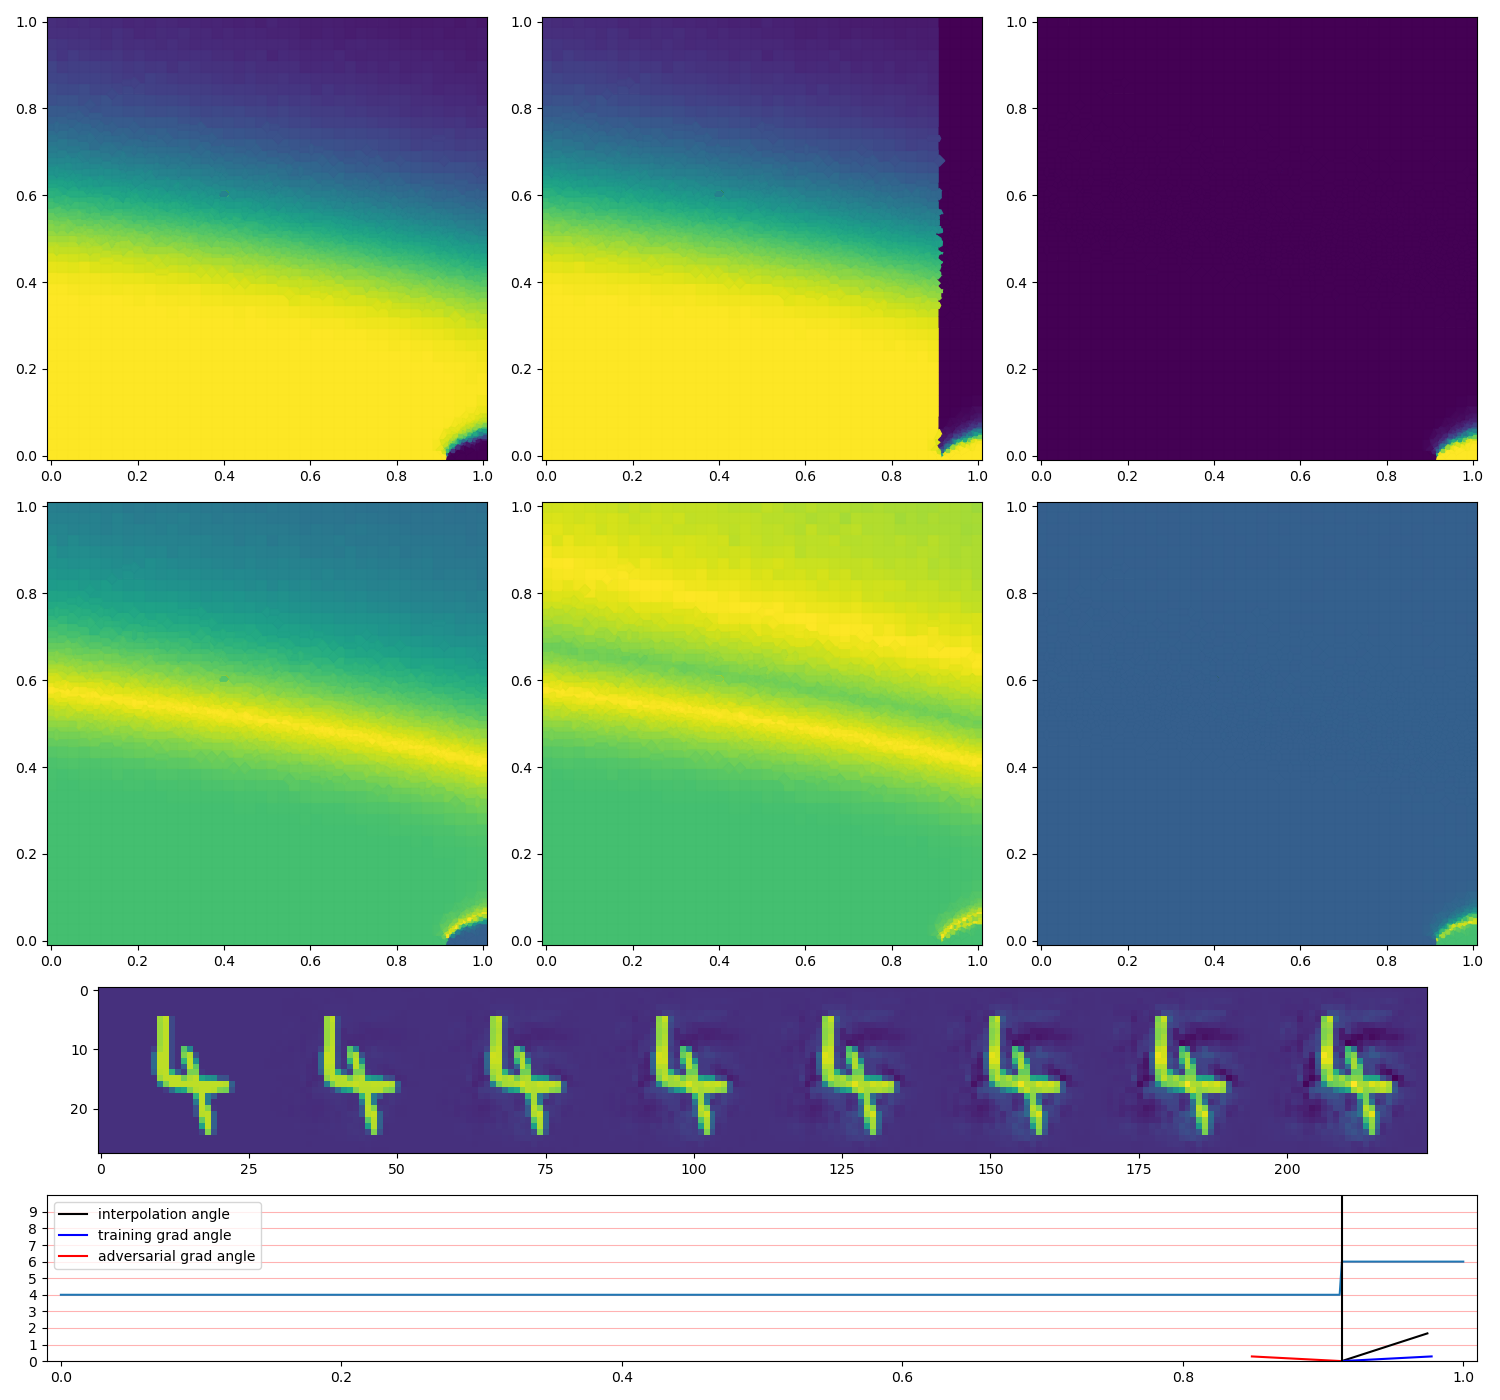
\includegraphics[width=0.42\textwidth]{c5_figures/stab-mnist-C32-50-50-10-0.001-eval-1e-06-pgd-4-6-db_interp-stability-50.png}
%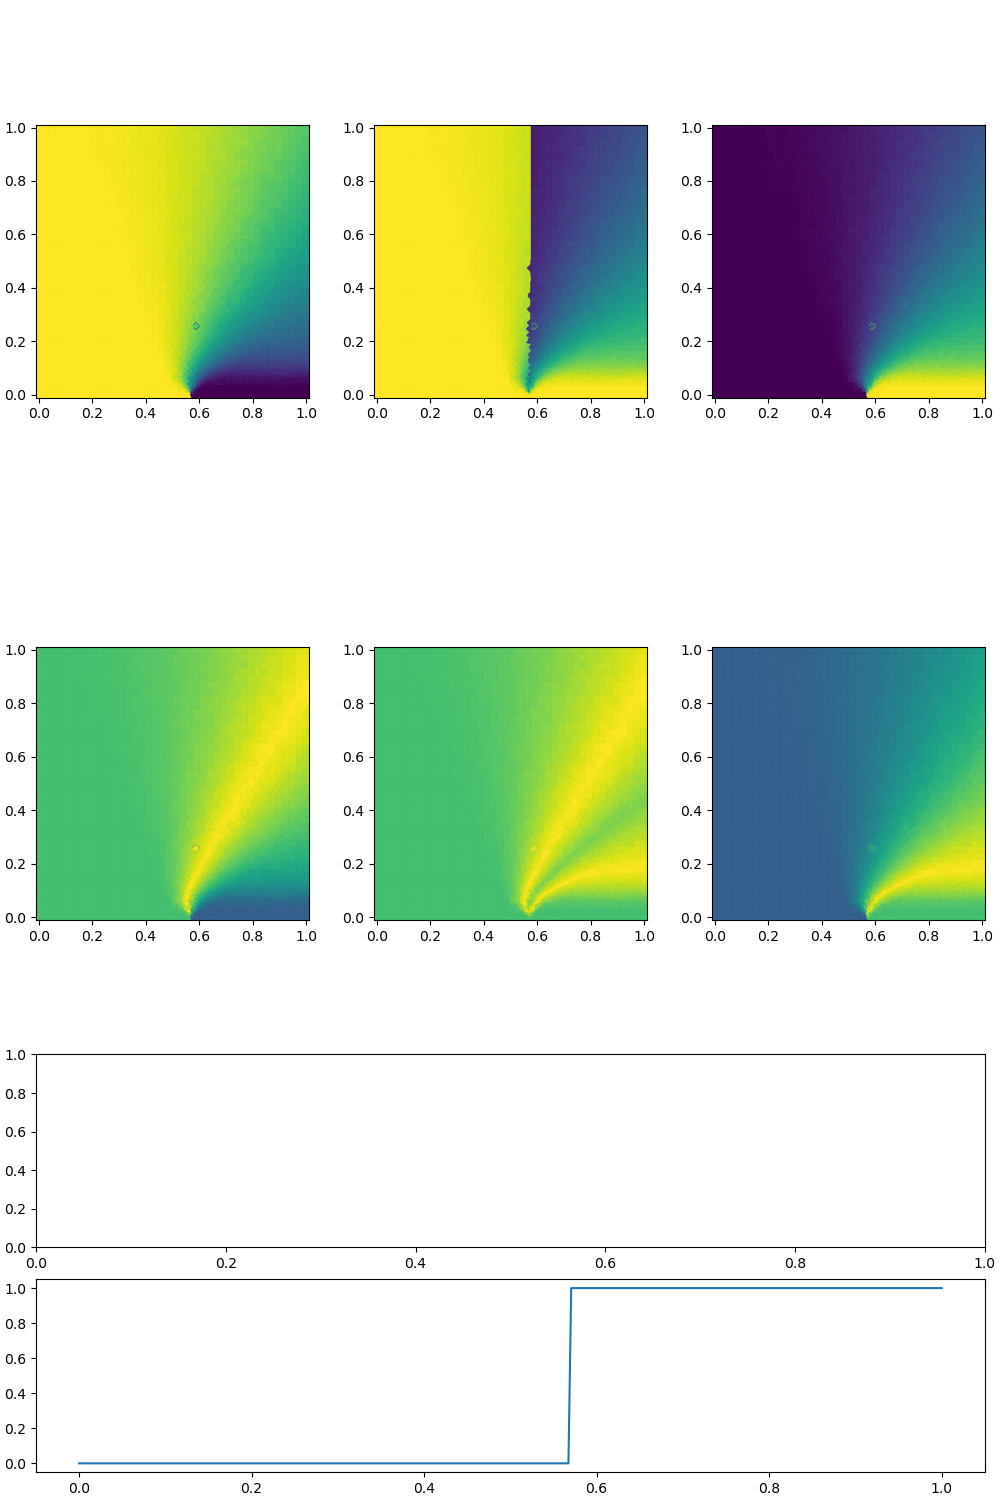
\includegraphics[width=0.9\textwidth]{c5_figures/wedge-mnist-C32-50-50-10-0.001-eval-1e-06-pgd-1-7-db_interp-stability-0.png}

    % 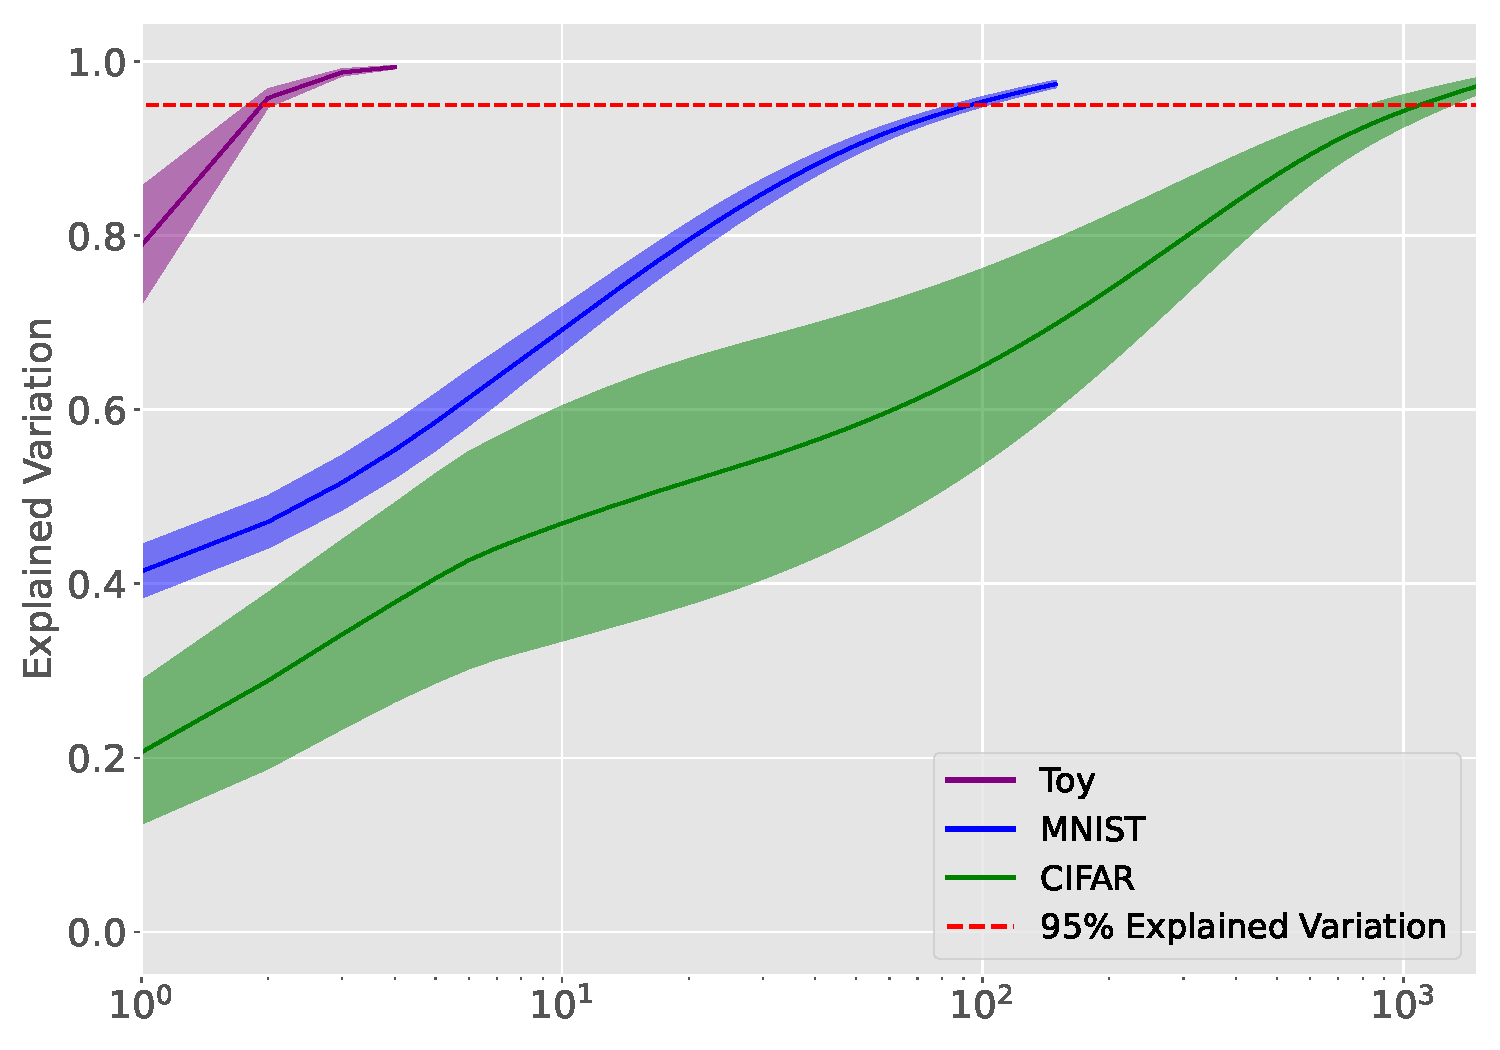
\includegraphics[width=0.45\textwidth]{c4a_figures/dimensionality_means.pdf}
    \caption{Heatmaps (top) and decision boundary angle plots bottom) showing stability fractions for an interpolation from a natural 4 to a natural 6 (left) and from a natural 4 to an adversarial 6 (right). }
    \label{fig:dbs}
\end{figure}


We can study persistence as a level-set in a sampling versus interpolation plot. We will design this approach using a Delaunay triangulation to iteratively sample this domain in order to visualize a decision boundary between natural images and between an adversarial image and a natural image. We will design heatmaps to show the fraction of uniform samples from a sphere which return the same class (E.g. an image along the interpolation for, say $t = 0.5$ is classified by the model as class 4. Then we will plot a column in the heatmap showing fraction of samples from Gaussians with progressively higher standard deviations which receive class 4.) This visualization is shown in Fig.~\ref{fig:dbs} where the middle  heatmaps show the 0.7 level set of these fractions, middle images show sample images along the linear interpolation across the decision boundary, and bottom plot shows incident angles on the decision boundary of the interpolant (black), the training gradient (blue) and the testing gradient (red). We can see that sharp geometric curvature and shallow angles are observed when interpolating across decision boundaries between natural and especially adversarial images. One line of future research will follow the direct geometric approach by constructing test objects (e.g. wedges which are intersections of angled hyper-planes forming arbitrarily sharp solids with arbitrarily many dimensions fewer than its ambient space) which replicate the structure observed in the practical networks. An example of this is shown in ~\ref{fig:dbs}.

      The second approach is to take advantage of the framework from Chapters ~\ref{Chapter4} and ~\ref{Chapter4a} in order to decompose the training gradients at points on the decision boundary to understand neural networks' learned degrees of freedom at these locations. The goal of this line of research is to understand these geometric constraints and eventually pose both updated training objectives and also better definitions for the identification of adversarial examples in practice. This line of research may have implications beyond robustness, to include uncertainty quantification, ability of models to generalize to data outside their training distribution, 
out-of-distribution detection, and other useful metrics to create
trustworthy AI. In particular, we can decompose adversarial gradients into an
initial gradient plus a component from each training input,
\begin{align}
  f(x, \theta_F) &= f(x, \theta_0) + \sum_i \sum_s \int_0^1 \langle
  \nabla_\theta f(x, \theta_s(t)), f(x_i, \theta_s(t))\rangle dt \\
  \dfrac{\partial f(x, \theta_F)}{\partial x} &= \dfrac{\partial f(x, \theta_0)}{\partial x} + \sum_i \sum_s \int_0^1 \langle
  \nabla_\theta \dfrac{\partial f(x, \theta_s(t))}{\partial x}, f(x_i,
                                 \theta_s(t))\rangle dt.
\end{align}
From this decomposition, we can also replace the individual training
data with an orthogonal basis by choosing vectors as in
~\citet{halko2011finding}, solving SVD for each step:
    Take a model, $f(x, \theta)$, which satisfies the necessary conditions for expression as:
 \begin{align}
     f(x, \theta_\text{tr}) &= f(x, \theta_0(0)) +  \sum_s
\int_0^1                                  \left\langle 
                                   \varphi_{s,t}(x) , \sum_i
                                   \left(L'(x_i, y_i) \varphi_{s,
                                   0}(x_i)\right) \right \rangle dt\\
     \varphi_{s,t}(x) &= \nabla_\theta f(x, \theta_s(t))
 \end{align}


Then we will let the RHS be rows of a matrix $L \cdot A$ where $X$ is a vector with elements $\varphi_{s,t}(x)$, $L =
$diag($L'(x_i, y_i))$ (size is $[N, N]$), and each row $A_i
= \varphi_{s,0}(x_i)$ so that $A$ has size $[N, P]$. Then we can compute $U\Sigma V^T =
A$ ($U$ of size $[N, P]$, $\sigma$ of size $[N, N]$, and $V^T$ of size $[P, P]$. Let's first try projecting each $A_i$ onto the row space of $V$ so that 
\begin{align}
    A_i &= \sum_k A_i V_k^T V_k \\
    \sum_i \left(L'(x_i, y_i) \varphi_{s, 0}(x_i)\right) = \sum_i L_i A_i &= \sum_i \sum_k L_i A_i V_k^T V_k\\
    \sum_i L_i A_i &= \sum_k \left(\sum_i L_i A_i V_k^T\right) V_k\\
    \sum_i L_i A_i &= \sum_k \left((\vec 1^T L A V^T)_k\right) V_k\\
\end{align}
where the subscripts all indicate rows. 
If we truncate  $V$ down to $K$ dimensions, then we have $B = \vec 1^T L A (V^K)^T$ with the matrices having sizes $[1,N], [N,N], [N,P], [P,K]$ (in order) and we can rewrite the truncated representation:

\begin{align}
    \sum_i L_i A_i &= \sum_k \left((\vec 1^T L A (V^K)^T)_k\right) V^K_k\\
    &= \sum_k B_k V^K_k.\\
\end{align}

Now, we can rewrite our original expression:
\begin{align}
     f(x, \theta_\text{tr}) &= f(x, \theta_0(0)) +  \sum_s
\int_0^1                                  \left\langle 
                                   \varphi_{s,t}(x) ,  \sum_k B_k V^K_k \right \rangle dt.
 \end{align}
More generally, we may define Fourier features along paths connecting all of the finitely many training steps together using methods like those from ~\citet{tancik2020fourierfeatures}. By combining these Fourier features spectral components across all training steps, it may be possible to perform a single spectral decomposition which provides a basis for the entire discrete path determined by a model during training. 

Regardless of how sophisticated we make this decomposition, all of
these methods have the advantage of maintaining an exact decomposition of predictions relative to contributions from each training input. This mapping implicitly
defines natural dimension reduction -- by truncating the chosen
basis. This provides a theoretical foundation
from which recent work in manifold study and data augmentation
~\citep{kaufman_data_2023, liu_linear_2023, sipka_differentiable_2023,
  cha_orthogonality-enforced_2023, marbut_reliable_2023,
  gao_out--domain_2023, oh_provable_2023, chen2023aware}.


\section{Generalization in the sense of Reproducing Kernel Banach Spaces}
Given that the representation from Chapter~\ref{Chapter4} and
~\ref{Chapter4a} have a small asymmetry, a general description of
these representations cannot fit within Hilbert Space. There is a
convenient approach building on the theory of Reproducing Kernel
Banach Spaces (RKBS) which is summarized nicely by
~\citet{zhang2009reproducing}. It is by careful construction of a
semi-inner product that I believe our representation can be written in
this way. This allows access to tools built for Banach spaces for
analysis of both accuracy, risk minimization, and other useful
results. A similar line of work is already being pursued by
~\citet{shilton_gradient_2023} with which our work can likely be
connected. Although this is less likely to produce practical
payoffs immediately, I believe that this approach will greatly enhance
the theoretical foundation upon which analysis of neural network
performance and limitations are based. 

\section{Connecting Distributional Learning with Neural Networks}

The neural representations and decompositions proposed in this work
provide images of the tangent space according to the
a given model for each point in the data space. The decomposed gradients for each input datum must be aligned with the natural geodesics which interpolate data. It has been shown increasingly in recent work
(e.g. by  ~\citet{lu2020universal}, ~\citet{yang2022capacity}, \citet{altekruger_neural_2023}) shows that Neural Networks
learn distributions in a sense that approximates the Wasserstein
metric to some order. Also, work by ~\citet{chizat2020maxmargin} that neural network
classifiers are approximately max-margin classifiers in some
implicit space. We cannot necessarily compute this space exactly,
however, by examining the parameter gradient decompositions exposed by this kernel representation, we can pose questions about this metric space in the
dual sense. Connecting these concepts into an
understanding of how Neural Networks embed an approximation of the
Wasserstein metric into euclidean space is likely
euclidean will have significant impact on the machine-learning
community at large. 



